

\chapter{VsnLib}                %crea il capitolo
%%%%%%%%%%%%%%%%%%%%%%%%%%%%%%%%%%%%%%%%%imposta l'intestazione di pagina
\lhead[\fancyplain{}{\bfseries\thepage}]{\fancyplain{}{\bfseries\rightmark}}
Strato di compatibilit\`a tra pacchetti netlink e stack di rete virtuali.

\section{Il Progetto}                 %crea la sezione
Gli stack analizzati in precedenza offrono a grandi linee la stessa tipologia di servizio seppur ognuna con le proprie caratteristice.\\
Nessuno dei progetti ha per\`o tenuto in considerazione l'idea di utilizzare un'interfaccia di configurazione che fosse standard e pertanto \`e necessario usare le funzioni specifiche per ognuno di questi progetti, costringendo il programmatore a cambiare modalit\`a di interazione da stack a stack.\\
Il progetto di creare questa libreria nasce proprio da questa esigenza, ovvero cercare di uniformare le interfacce di comunicazione in modo tale che l'utente non sia costretto ad adattarsi ogni qual volta decida di cambiare stack.\\
\section{VnsLib}
\subsection{Preambolo}
Per configurare uno stack di rete programmi come ip generano un pacchetto netlink con le informazioni necessarie lo inviano al kernel che lo elabora esegue le operazioni e genera un messaggio di errore nel quale esiste un flag contenente il numero di errore generato (0 in caso di successo), a questo messaggio \`e associato un payload di risposta che pu\`o essere usato per generare un feedback da mostrare all'utente che sta interagendo con il programma.\\
VsnLib \`e un progetto in fase di sviluppo scritto in C e completamente opensource, liberamente scaricabile attraverso la piattaforma github al seguente link \url{https://github.com/simonepreite/vsnlib}.

\subsection{Ambiente}
La necessit\`a primaria era quella di catturare queste comunicazioni netlink e per farlo la strada era quella di intercettare la system call di invio della richiesta contenente appunto il payload, questo momento \`e quello in cui viene eseguita la sendto.\\
In questo punto interviene la nostra libreria, che si interpone e di fatto fa le veci del kernel, al quale il pacchetto netlink non arriver\`a mai realmente.\\
Il progetto inizialmente utilizzava come motore di cattura delle system call la libreria purelibc\footnote{http://wiki.virtualsquare.org/wiki/index.php/PureLibc}, in seguito per\`o si \`e giunti alla conclusione che costruire un modulo ad hoc all'interno del sistema vuos fosse un'alternativa pi\`u versatile, immediata e pulita, inoltre vuos ha un sistema di debug built in che rende pi\`u semplice l'individuazione dei problemi legati allo sviluppo.\\
Il modulo in questione si chiama unrealvsnlib per analogia alla libreria ma ognuno potrebbe costruire un suo modulo a seconda di quello che intende controllare.\\

\subsection{Core}
La libreria costituisce uno strato  intermedio di compatibilit\`a tra netlink e le specifiche configurazioni degli stack.\\
Vediamo come \`e composta:
\begin{description}                     %crea un elenco descrittivo
  \item[VnsLib:] Il primo stato si occupa di inizializzare la libreria in base allo stack che si intende utilizzare, in questo modo possiamo caricare dinamicamente solo il modulo che ci interessa.
  \item[Modules:] Sono la parte specifica della libreria, essi contengono l'intestazione delle funzioni generiche che si occupano di chiamare quelle particolari per ogni stack.
\end{description}
\begin{figure}[h]                       %crea l'ambiente figura; [h] sta
                                        %   per here, cio� la figura va qui
\begin{center}                          %centra nel mezzo della pagina
                                        %   la figura
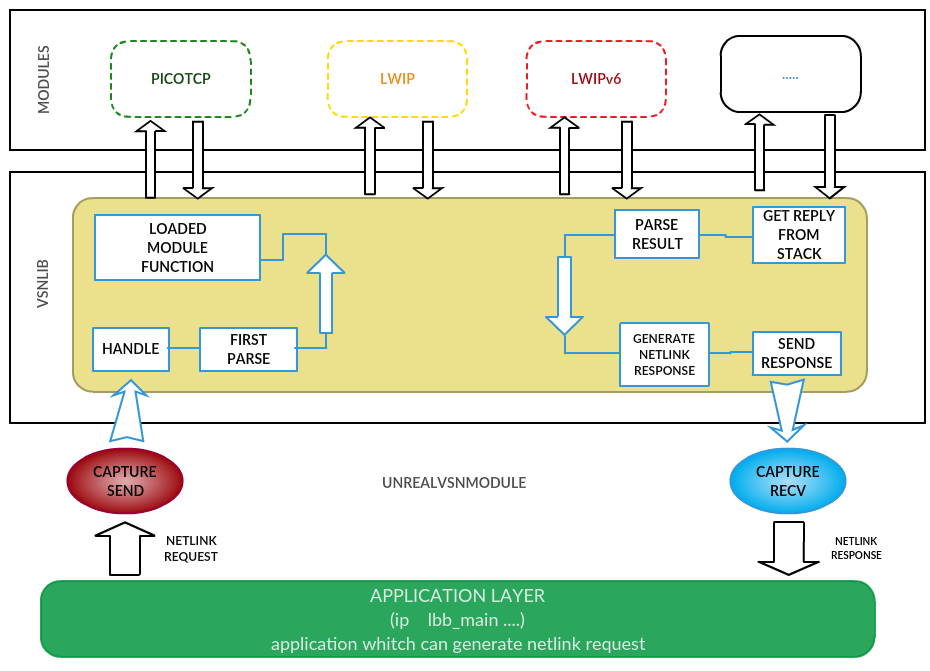
\includegraphics[width=16cm]{vsnlib_scheme}%inserisce una figura larga 5cm
                                        %se si vuole usare va scommentata
%
%%%%%%%%%%%%%%%%%%%%%%%%%%%%%%%%%%%%%%%%%inserisce la legenda ed etichetta
                                        %   la figura con \label{fig:prima}
\caption[mappa concettuale libreria]{mappa concettuale libreria}\label{fig:map}
\end{center}
\end{figure}
\subsection{VnsLib}
Espone le interfacce di comunicazione della libreria, che di fatto sono due, una per inizializzare l'ambiente ed una per inviare il pacchetto da gestire.\\
L'utente non ha accesso ad altre funzioni perch\`e \`e la libreria stessa ad analizzare il pacchetto, riempire i campi della struttura generica ed inviarlo al modulo relatvo allo stack.\\
Di ritorno si ricever\`a una struttura che permetter\`a la costruzione del paccehetto netlink di risposta alla recv del programma, questo \`e l'ultimo compito della nostra libreria.
\subsection{Moduli}
La potenza dei moduli risiede nel fatto che chiunque abbia intenzione di costruire uno stack personalizzato, o di utilizzarne uno per il quale non esiste un modulo, pu\`o facilmente realizzare il proprio e la libreria si occuper\`a di farne il caricamento qualora fosse richiesto.
Ogni modulo, infatti, ha la stessa struttura e contiene una funzioni generiche comuni in tutti gli stack. I prototipi di queste funzioni hanno in comune la desinenza che serve a specificare l'azione da compiere, mentre a distinguerle \`e la radice che prende il nome dello stack, pertanto ogni modulo \`e composto dallo stesso numero di funzioni che si occupano mediare la comunicazione tra la libreria e il vero stack. Questa mediazione non \`e particolarmente complessa da comprendere in quanto si tratta di una semplice sequenza di chiamate alle funzioni specifiche dello stack per realizzare l'azione della richiesta.\\
Per generalizzare la libreria si \`e usata una tecnica di puntatori a funzione, in questo modo possiamo evitare di specificare il nome completo delle funzioni che, come gi\`a accennato si differenziano per nome. Allora l'idea \`e stata quella di inizializzare, in fase di caricamento della libreria (che avviene con dlopen), proprio un array di puntatori a funzione (attraverso dlsym) in modo tale da poter effettuare le chiamate attraverso di esso. Questo sistema ci permette di caricare dinamicamente solo il modulo di cui si necessita.\\
Ogni funzione riceve lo stesso tipo di struttura e dopo aver raccolto i risultati delle funzioni specifiche dello stack riempie i campi utili a formare la struttura di risposta che poi sar\`a ritornata alla libreria per elaborare il pacchetto netlink di risposta.
\section{Sviluppi Futuri}
In fase di progettazione non sono stati posti limiti alla crescita del progetto e la sua modularit\`a \`e legata principalmente a questo aspetto.\\
L'augurio \`e che questo progetto continui a crescere arricchendosi di funzionalit\`a.\\
In questa fase ci si \`e occupati delle configurazioni e del routing che deve essere completata e testata prima di poter affermarne la stabilit\`a.\\
Tra le varie ipotesi di proseguimento c'\`e quella di gestione del filtering ovvero occuparsi di tutta la parte riguardante le iptables.
%%%%%%%%%%%%%%%%%%%%%%%%%%%%%%%%%%%%%%%%%non numera l'ultima pagina sinistra
\clearpage{\pagestyle{empty}\cleardoublepage} 
